\documentclass[10pt,a4paper]{article}
\usepackage[utf8]{inputenc}
\usepackage{amsmath}
\usepackage{amsfonts}
\usepackage{amssymb}
\usepackage{pgf-umlcd}
\usepackage{tabularx}
\usepackage{pdflscape}
\usepackage[obeyspaces]{url}
\usepackage{float}
\usepackage{framed}
\usepackage[linesnumbered]{algorithm2e}
\usepackage{cprotect}
\newcolumntype{Y}{>{\centering\arraybackslash}X}
\usepackage{graphicx}
\usepackage{subfigure}
\newcommand{\dsb}[1]{[\![#1]\!]}
\usepackage{adjustbox}
\usepackage[nottoc,numbib]{tocbibind}

\author{Myles Lee}
\title{Repository Knowledge Transfer in Automatic Optimisation of Reconfigurable Designs}
\begin{document}

\maketitle
This project was supervised by Maciej Kurek and Wayne Luk and managed under the UROP scheme at the Custom Computing Group at the Department at Computing in Imperial College London.

\tableofcontents

\section{Introduction}
This project adapts the cost-aware, constrained, global, non-convex mathematical optimisation problem to the reconfigurable computing domain. The objective is to optimise a design $T$, by finding the optimal configuration $\mathbf{x}_T^*$ of a fitness function $f_T$, with a budget of $f_T$ evaluations. $T$ has $n_T$ reconfigurable parameters. The design space $\mathbb{X}_T$ is defined to be the Cartesian product of $n_T$ intervals. $f_T$ is expensive to evaluate and cannot be assumed that $f_T$ is differentiable or convex. Therefore, computing $\mathbf{x}_T^*$ is expensive. Finding the optimal design maybe too costly, and a sub-optimal configuration may be used.

Each design has a label function $g_T$, such that for some configuration $\mathbf{x}$, $g_T(\mathbf{x})=0$ if and only if $\mathbf{x}$ is successful. $g_T(\mathbf{x}_T^*)=0$ is required. In addition, each design have $h_T$ constraint functions $\{{\mathbf{h}_1}_T,...\}$. Each constraint function determines the resource restrictions on the configurations. In the reconfigurable computing context, a constraint function could represent the fraction of used hardware resource on the chip. For some constraint function ${\mathbf{h}_i}_T$ and configuration $\mathbf{x}$, ${\mathbf{h}_i}_T(\mathbf{x})<1$ if and only if $\mathbf{x}$ satisfies the $i^{\text{th}}$ constraint. Therefore $\forall \mathbf{x}\in\mathbb{X}_T.(\forall i\in\{1,...,h_T\}.{\mathbf{h}_i}_T(\mathbf{x})<1)\Leftrightarrow g_T(\mathbf{x})=0$.

Moreover, each design have $c_T$ cost functions, where each cost function determines the cost of evaluating a component of $f_T$. For example, two cost functions can represent the software and hardware build time. Typically, the cost is defined as the time taken to evaluate $f_T$. The cost of evaluating $f_T(\mathbf{x})$ is the sum of each cost function, $\sum_{i=1}^{c_T}{\mathbf{c}_i}_T(\mathbf{x})$. The budget restricts the number of $f_T$ evaluations, as the sum of evaluation costs must not exceed the budget. If the evaluation cost of any configuration is constant, then the budget can be interpreted as a scale of the maximum number of $f_T$ evaluations.

To minimise this cost, a pre-optimised source design $S$ can be used to provide insight to a target design $T$ with limited sampling. Using observations from $f_S$, $\mathbf{x}_T^*$ can be approximated from $\mathbf{x}_S^*$. Knowledge transfer is used to estimate properties of $T$ using other, possibility similar designs such as $S$.

\section{Contributions}

The main contributions of this project are summarised below:
\begin{enumerate}
\item Improvement of the surrogate to predict $f_T$, using a \emph{Transferable Gaussian Process}
\item Extension of knowledge transfer to predict a near-optimal configuration at the first evaluation
\item Extension of knowledge transfer using a repository consisting of multiple designs
\item Modification of previous code base\cite{Nicholson2015} with implementation of the above concepts
\end{enumerate}
\subsection{Transferable Gaussian Process}

Previous effort\cite{Kurek2016} used a polynomial function $z$ to map from source to target fitness values such that $z\circ f_S\approx f_T$. This is derived from polynomial regression of sampled source and target fitness values. However, $z$ is inaccurate for predicting when $f_S$ and $f_T$ are noisy or high dimensional functions. An example follows to demonstrate this.

Suppose $f_S(\mathbf{x})=1+\mathbf{x}_1$, $f_T(\mathbf{x})=1+\mathbf{x}_1+\mathbf{x}_2$ and $\mathbb{X}_S=\mathbb{X}_T=[0,1]^2$. By sampling at $\{(0,0),(0,1),(1,0),(1,1)\}$, we obtain the observations $\{((0,0),1),\allowbreak((0,1),1),\allowbreak((1,0),2),((1,1),2)\}$ and $\{((0,0),1),((0,1),2),((1,0),2),((1,1),3)\}$ by evaluating $f_S$ and $f_T$ respectively. By pairing source and target sample points, we obtain $\{(1,1),(1,2),(2,2),(2,3)\}$. Using linear regression, we can derive $z(y)=\frac{1}{2}+y$. Then for some sample, $(z\circ f_S)(x_1,x_2)=\frac{3}{2}+x_1\not=f_T(x_1,x_2)$. Therefore $z$ is inaccurate.

To solve this, a Transferable Gaussian Process (TGP) is used as follows. A TGP is composed of two Gaussian Processes of the same kernel, a process $p$ to predict the scalar of $f_S$ to $f_T$ and process $q$ as a surrogate of $f_T$. $p$ is trained on the ratio of source and target fitness values, so $p(\mathbf{x})=\frac{f_T(\mathbf{x})}{f_S(\mathbf{x})}$ at sampled points. The training data for the example above would be $\{((0,0),1),((0,1),2),((1,0),1),\allowbreak((1,1),\frac{3}{2})\}$. $q$ is trained on the observations of $f_S$, so $q=f_S$ at sampled points. Then we define $z(\mathbf{x})=p(\mathbf{x})q(\mathbf{x})$. So $(z\circ f_S)(\mathbf{x})=\frac{f_T(\mathbf{x})}{f_S(\mathbf{x})}\cdot f_S(\mathbf{x})=f_T(\mathbf{x})$. Using TGPs are more accurate than using polynomial regression because TGPs captures transferred features better in high dimensional space.

\subsection{Near-optimal Configuration Prediction}
Correlation analysis is used to determine the effectiveness of predicting a near-optimal configuration. For each dimension $i$ of the $\mathbb{X}_S$, we compute the Spearman correlation coefficient $\rho_i$ by comparing configurations against fitness values using observations of $f_S$. For a given significance level $\alpha$, if $\forall i\in\dsb{1,n_S}.1-|\rho_i|\le\alpha$ and $n_S=n_T$, then we can apply knowledge transfer. We approximate $f_S$ with a multi-dimensional quadratic function $\hat{f_S}$\cite{Xi2004}. We use multi-linear regression to find constants $c$, $\mathbf{d}$ and $\mathbf{e}$ such that $\hat{f_S}(\mathbf{x})=c+\sum_{i=1}^{n_S}\mathbf{d}_i \mathbf{x}_i+\mathbf{e}_i \mathbf{x}_i^2$. Then we approximate $\mathbf{x}_T^*\approx argmin_{\mathbf{x}\in\mathbb{X}_T}\hat{f_S}(\mathbf{x})$. This approximation is a signifiant improvement over using $\mathbf{x}_T^*\approx\mathbf{x}_S^*$ because $f_T$ and $f_S$ tend to be noisy and independent in each dimension. The evaluation section illustrates this improvement.

\subsection{Repository Knowledge Transfer}

We know how to apply knowledge transfer from one source design to a target design. To apply knowledge transfer from multiple sources, we need to select a design from the repository that has the highest transferability to optimise the target design. Formally, let the repository $R$ be the set of source designs $\{S_1,...\}$. Let $f_{transferability}$ measure the transferability of using knowledge transfer from $S$ to $T$. The objective is to find $argmax_{S\in R}f_{transferability}(S,T)$.

We extend designs to include parameter names and tags. For an arbitrary design $T$, parameter names $names_T$ label each reconfigurable parameter. As different designs may share the same parameter names, we may be able to derive common properties of these designs. For example, decreasing the mantissa width generally decreases the accuracy for any design. $T$ is associated with tags $tags_T$, which describes high-level keywords, such as ``uses square root'' and ``implements matrix multiplication''.

\[
	\begin{split}
		f_{transferability}(S,T)=f_{names}(S,T)\times(f_{common}(S,T)+\frac{1}{|f_{cross}(S,T)|}\\
			+f_{boundaries}(S,T)+f_{tags}(S,T))
	\end{split}
\] where
\[f_{names}(S,T)=|names_S\cap names_T|\]
\[f_{common}(S,T)=\text{number of common points in $O_S$ and $O_T$}\]
\[
	\begin{split}
		f_{cross}(S,T)=\text{standardized cross-validated residual\cite{Jones1998}}\\
			\text{of predictor Gaussian process in TGP}
	\end{split}
\]
\[f_{boundaries}(S,T)=\frac{|\mathbb{X}_S\cap\mathbb{X}_T|}{|\mathbb{X}_T|}\]
\[f_{tags}(S,T)=|tags_S\cap tags_T|\]

The intuition of the definition of $f_{transferability}$ is derived by visualising each design on a hypergraph $G$. For each design in $R\cup\{T\}$, let each unique name and the set of names be a node and a hyperedge in $G$ respectively. If the hyperedges of two designs $S_1$ and $S_2$ intersect, then the number of intersecting nodes is $f_{names}(S_1,S_2)$. We only want to compare designs that have common names with $T$. Hence, $f_{names}(S,T)=0\Rightarrow f_{transferability}(S,T)=0$. Note that $f_{transferability}(S,T)$ is maximised when $S=T$. If $S=T$ then, we can optimise $S$ to find $\mathbf{x}_S^*$, to directly infer $\mathbf{x}_T^*$.

\subsection{Modification of Codebase}

For the full details of modifications, refer to the Git repository of the accompanying source code. The main changes are summarised as below:
\begin{enumerate}
	\item Implemented knowledge transfer
	\item Replaced the particle swarm optimiser with a simplifed global Nelder Mead optimiser\cite{Luersen2004}
	\item Removed asynchronous features
	\item Replaced Python script interface with an Evaluator class that interfaces with arbitrary scripts 
\end{enumerate}

The implementation of knowledge transfer follows the algorithm below. For the full details, see \path{transferrer.cpp}. We use $10n_T$ samples\cite{Jones1998} to learn about $T$, by using $5n_T$ configurations from $S$ to sample $T$ and using $5n_T$ configurations from LHS in the EGO algorithm. 
\begin{figure}[H]
	\begin{framed}
		\begin{algorithm}[H]
			Let $O_S$ and $O_T$ be observations from $S$ and $T$ respectively\\
			Filter $O_S$ if observation exceeds fitness percentile threshold $\beta$\\
			\If{$O_S$ is sufficently independent with significance level $\alpha$}{
				Compute multi-quadratic regression $\hat{f_S}$ from $O_S$\\
				$\mathbf{x}_q=argmin_{\mathbf{x}\in\mathbb{X}_S}\hat{f_S}(\mathbf{x})$\\
				$\mathbf{y}=(f_T(\mathbf{x}_q),g_T(\mathbf{x}_q),{\mathbf{h}_1}_T(\mathbf{x}_q),...,{\mathbf{c}_1}_T(\mathbf{x}_q),...)$\\
				Add $(\mathbf{x},\mathbf{y})$ to $O_T$
			}
			Select $5n_T$ successful configurations randomly from $O_S$ into $\mathbf{X}$\\
			\For{$\mathbf{x}\in\mathbf{X}$}{
				$\mathbf{y}=(f_T(\mathbf{x}),g_T(\mathbf{x}),{\mathbf{h}_1}_T(\mathbf{x}),...,{\mathbf{c}_1}_T(\mathbf{x}),...)$\\
				Add $(\mathbf{x},\mathbf{y})$ to $O_T$
			}
			Construct TGPs using $O_S$ and $O_T$\\
			Run EGO algorithm with TGPs
		\end{algorithm}		
	\end{framed}
	\caption{Single-source knowledge transfer algorithm}
\end{figure}

\section{Evaluation}

\subsection{Designs}

Knowledge transfer was used to improve the optimisation of porting reconfigurable designs from the Max3 to the Max4 platform.

\begin{table}[H]
	\begin{tabularx}{\linewidth}{X l Y c c X}
		\hline
		Design & Platform & $\mathbb{X}$ & $h$ & $c$ & $names$\\
		\hline
		robot\cite{Chau2014} & & $\{2^n|n\in\dsb{1,4}\}\times\dsb{10,40,2}\times\dsb{2048,8168,60}$ & 4 & 1 & cores, mantissa width, particles\\
		stochastic\cite{Chau2014} & & $\{2^n|n\in\dsb{1,4}\}\times\dsb{10,40,2}\times\dsb{96,4056,60}$ & 4 & 1 & cores, mantissa width, particles\\
		quadrature\cite{Tse2012} & Max3 & $\dsb{1,24}\times\dsb{4,32}\times\dsb{11,53}$ & 1 & 1 & cores, density factor, mantissa width\\
		quadrature\cite{Tse2012} & Max4 & $\dsb{1,16}\times\dsb{4,32}\times\dsb{32,53}$ & 1 & 0 & cores, density factor, mantissa width\\
		xinyu rtm\cite{Niu2012} & Max3 & $\dsb{1,10}\times\dsb{1,10}\times\dsb{4,24}\times\dsb{1,3}\times\dsb{1,10}\times\dsb{1,10}\times\dsb{1,32}$ & 0 & 1 & alpha, beta, B, T, Pknl, Ptl, Pdp\\
		xinyu rtm\cite{Niu2012} & Max4 & $\dsb{1,10}\times\dsb{1,10}\times\dsb{4,24}\times\dsb{1,3}\times\dsb{1,20}\times\dsb{1,20}\times\dsb{1,32}$ & 0 & 1 & alpha, beta, B, T, Pknl, Ptl, Pdp\\
		genomics\cite{Arram2017} & Max3 & $\dsb{1,10}\times\dsb{-3,3}\times\dsb{0,1}$ & 0 & 1 & sample distance, optimisation index, oversample\\
		genomics\cite{Arram2017} & Max4 & $\dsb{1,10}\times\dsb{-3,3}\times\dsb{0,1}$ & 0 & 1 & sample distance, optimisation index, oversample\\
		\hline
 	\end{tabularx}
	\caption{Designs used for knowledge transfer}
\end{table}

\begin{figure}[H]
	 \begin{center}
		\subfigure[quadrature Max3 cores=1]{
			\includegraphics[width=0.45\textwidth]{images/quadrature_max3_fitness.png}
		}
		\subfigure[quadrature Max4 cores=1]{
			\includegraphics[width=0.45\textwidth]{images/quadrature_max4_fitness.png}
		}
		\subfigure[genomics Max3 oversample=0]{
			\includegraphics[width=0.45\textwidth]{images/genomics_max3_oversample_0_fitness.png}
		}
		\subfigure[genomics Max3 oversample=1]{
			\includegraphics[width=0.45\textwidth]{images/genomics_max3_oversample_1_fitness.png}
		}
		\subfigure[genomics Max4 oversample=0]{
			\includegraphics[width=0.45\textwidth]{images/genomics_max4_oversample_0_fitness.png}
		}
		\subfigure[genomics Max4 oversample=1]{
			\includegraphics[width=0.45\textwidth]{images/genomics_max4_oversample_1_fitness.png}
		}
	\end{center}
	\caption{Function surface plots of designs}
	\label{fig:subfigures}
\end{figure}

\subsection{Optimisation}

\begin{figure}[H]
	 \begin{center}
		\subfigure[robot to stochastic]{
			\includegraphics[width=0.45\textwidth]{images/robot_stochastic_optimisation.png}
		}
		\subfigure[stochastic to robot]{
			\includegraphics[width=0.45\textwidth]{images/stochastic_robot_optimisation.png}
		}
		\subfigure[quadrature Max3 to Max4]{
			\includegraphics[width=0.45\textwidth]{images/quadrature_max3_max4_optimisation.png}
		}
		\subfigure[genomics Max3 to Max4]{
			\includegraphics[width=0.45\textwidth]{images/genomics_max3_max4_optimisation.png}
		}
		\subfigure[xinyu rtm Max3 to Max4]{
			\includegraphics[width=0.45\textwidth]{images/xinyu_rtm_max3_max4_optimisation.png}
		}
	\end{center}
	\caption{Optimisation graphs illustrating knowledge transfer improvement}
	\label{fig:subfigures}
\end{figure}

Each knowledge transfer application has been executed 1000 times. In the optimisation graphs, the solid lines represent the mean of best fitness values and the shaded area represents the confidence interval of one standard deviation from the mean. Each application results in a non-increasing curve. This function is not defined for all evaluations because evaluated points may not meet the design's constraints, hence there is no fitness value. Therefore, taking an aggregate of these functions does not necessarily result in a non-increasing function, as shown in the optimisation of the xinyu rtm Max4 design.

From the optimisation graphs, we observe that using knowledge transfer results in faster optimisation. When the optimal configuration is at the edge of the configuration space, the near-optimal configuration prediction is very effective. This is evident in the quadrature and genomics examples where the first evaluations are near-optimal. When a fitness surface function is more noisy, then the optimisation function is more uncertain, as in the robot example. This is due to the inaccuracy of interpolation using a few observations.

The key result was the optimisation of genomics designs. The fitness is the benchmark execution time to run the DNA exact alignment and the cost is the time taken to build each design. The optimisation index is a combination of the step size and precomputed interval parameters. Because these parameters are mutually-exclusive, the dimension of the configuration space can be reduced.

\subsection{Quantification of Improvement}

To quantify the improvement of using knowledge transfer, let the number of knowledge transfer applications be $\lambda$. Define a scoring function $score$ on the $i^{\text{th}}$ optimisation function $f_i:\mathbb{R}_{\ge 0}\rightharpoonup\mathbb{R}$ for some $i\in\dsb{1,\lambda}$, that gives the best fitness value given some cost utilisation $t$.

\[
	\begin{split}
		score(f_i)&=\dfrac{1}{t_{max}(y_{max}-y_{min})}\\
		&\int_{t=0}^{t_{max}}min\{f_i(j)|j\in[0,t],\exists y\in\mathbb{R}.f_i(j)=y\}\cup\{y_{max}\}-y_{min}\mathrm{d}t
	\end{split}
\]where
\[y_{min}=min\{f_i(t)|i\in\dsb{1,\lambda},t\in\mathbb{R},\exists y\in\mathbb{R}.f_i(t)=y\}\]
\[y_{max}=max\{f_i(t)|i\in\dsb{1,\lambda},t\in\mathbb{R},\exists y\in\mathbb{R}.f_i(t)=y\}\]
\[t_{max}=max\{t|i\in\dsb{1,\lambda},t\in\mathbb{R},\exists y\in\mathbb{R}.f_i(t)=y\}\]

Intuitively, $score$ defines the normalised area under the optimisation graph. The complication arises because $f_i$ is not a total function. The formula is derived by summing the regret $f_i(t)-y_{min}$ as the cost $t$ increases. A score of zero means that the optimiser selects the optimal configuration with no cost, hence no regret. A score of one means the optimiser does not improve from the worst configuration, or does not select any successful configurations. To account for the randomicity of the optimiser, we take the average of $score(f_i)$ for each $i$. The improvement of using knowledge transfer is the ratio of the average score without knowledge transfer divided by the average score with knowledge transfer.

A limitation of the definition of $score$ is that this definition does not describe the distribution of $f_i$. However, the balance between quickly finding a near-optimal configuration and slowly finding a optimal configuration is not well-defined. An alternative definition would be the cost required to achieve the optimal configuration, but this is not suitable for large configuration spaces as the cost of finding the optimal configuration varies greatly or the optimal configuration is not found

\begin{table}[H]
	\begin{tabularx}{\linewidth}{X X X X X}
		\hline
		$T$ & $S$ & No KT Score & KT Score & Improvement Ratio\\
		\hline
		robot & stochastic & 0.165 & 0.164 & $\phantom{0}$1.001\\
		stochastic & robot & 0.276 & 0.230 & $\phantom{0}$1.198\\
		quadrature Max3 & quadrature Max4 & 0.077 & 0.053 & $\phantom{0}$1.452\\
		genomics Max3 & genomics Max4 & 0.020 & 0.009 & $\phantom{0}$2.269\\
		xinyu rtm Max3 & xinyu rtm Max4 & 0.560 & 0.013 & 44.481\\
		\hline
	\end{tabularx}
	\caption{Scores of knowledge transfer applications}
\end{table}

\subsection{Repository}

For each target design, the repository knowledge transfer selects the most suitable source design from the repository automatically. If the repository includes the target design, the target design is always selected for transfer.
\section{Technical Documentation}

The program is written in C++ 14. Each design mentioned in the evaluation section can be found in the \path{examples} directory. The program has the dependencies: \path{Catch}, \path{eigen}, \path{gsl}, \path{ihs} and \path{libgp}.

\subsection{Structure}

\begin{table}[H]
	\begin{tabularx}{\linewidth}{l X}
		\hline
		File/Directory & Description\\
		\hline
		\path{animation} & manages the printing of animated progress messages to standard output\\
		\path{catch} & unit test library\\
		\path{csv} & manages file I/O with CSV files\\
		\path{compare} & comparison metrics between source designs and a target design\\
		\path{eigen3} & libgp dependency\\
		\path{ego} & efficient global optimiser\\
		\path{evaluator} & interfaces command line script with runtime variables and caches results\\
		\path{examples} & directory of designs used for benchmarking\\
		\path{functions} & collection of general functions\\
		\path{gsl-2.4} & GNU scientific library\\
		\path{gp} & wrapper for libgp's Gaussian processes with log-space and whitening transformation\\
		\path{ihs} & hypercube sampling library\\
		\path{logs} & directory of experiment results\\
		\path{Makefile} & builds and tests executable\\
		\path{tgp} & implementation of TGP\\
		\path{transferrer} & implementation of single knowledge transfer that wraps EGO\\
		\path{scripts} & Bash and Python scripts to manage batch execution and manipulate CSV files\\
		\path{surrogate} & interface for high dimensional regression\\
		\hline
	\end{tabularx}
	\caption{Files and directories descriptions in the working repository}
\end{table}
\begin{landscape}
	\begin{tabularx}{\linewidth}{l X X}
		\hline
		Name & Description & Example\\\hline
		\path{run_experiments_all.py} & runs program on all precomputed examples with and without knowledge transfer & \path{./scripts/run_experiments_all}\\
		\path{run_experiments.py} & runs program on source and target designs with and without knowledge transfer & \path{./scripts/run_experiments examples/robot examples/stochastic 5}\\
		\path{compare_experiments.py} & computes optimisation statistics from logs with and without knowledge transfer & \path{python3 scripts/compare_experiments.py examples/robot/ examples/stochastic/}\\
		\path{csv_stats.py} & computes statistics on a CSV file & \path{python3 scripts/csv_stats.py examples/robot/results.csv}\\
		\path{fill_space.py} & adds failed builds to precomputed results when results do not exhaustively represent the configuration space & \path{python3 scripts/fill_space.py examples/robot/results.csv 1 4 8 40}\\
		\path{lookup.py} & given a configuration as command-line parameters, uses a CSV file as a lookup table & \path{python3 scripts/lookup.py examples/robot/results.csv 1 8}\\
		\path{parser.py} & aggregates results by computing average fitness value of each duplicate sampled point & \path{python3 scripts/parser.py examples/robot/results.csv 2}\\
		\path{plot_experiments.py} & plots optimisation curve with and without knowledge transfer & \path{python3 scripts/plot_experiment.py examples/robot/ examples/stochastic/}\\
		\path{plot_results.py} & plots 2-dimensional fitness function surface & \path{python3 scripts/plot_results.py examples/robot/config.txt examples/robot/results.csv output.png}\\
		\path{run_example} & runs program on a example design without knowledge transfer & \path{./scripts/run_example examples/robot}\\
		\path{transfer_example} & runs program on a target example design with knowledge transfer using a source & \path{./scripts/transfer_example examples/robot examples/stochastic}\\
	\end{tabularx}
	\begin{table}[H]
		\begin{tabularx}{\linewidth}{l X X}
			\path{transfer_repository} & recommends a source design for knowledge transfer\ & \path{./scripts/transfer_repository examples/robot}\\
			\path{transfer_repository_all} & checks that all recommended source designs are most suitable for knowledge transfer across all example designs & \path{./scripts/transfer_repository_all}\\
			\hline
		\end{tabularx}
		\cprotect\caption{Scripts in the \path{script} directory}
	\end{table}
\end{landscape}

\begin{figure}[H]
	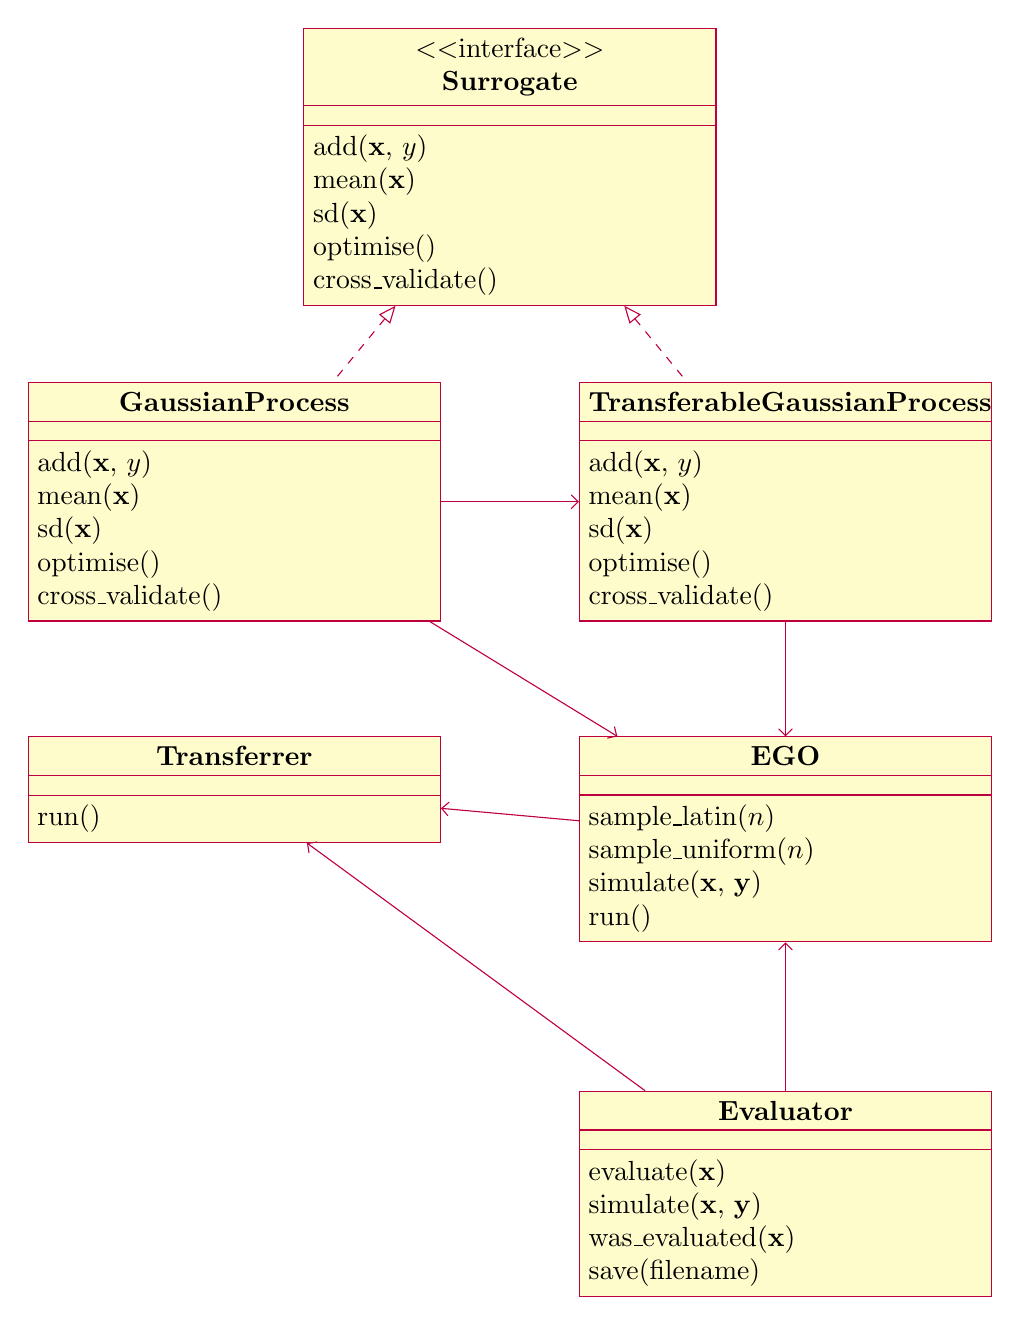
\begin{tikzpicture}
		\begin{interface}{Surrogate}{0 ,0}
			\operation{add($\mathbf{x}$, $y$)}
			\operation{mean($\mathbf{x}$)}
			\operation{sd($\mathbf{x}$)}
			\operation{optimise()}
			\operation{cross\_validate()}
		\end{interface}
		
		\begin{class}{GaussianProcess}{-3.5, -4.5}
			\implement{Surrogate}
			\operation{add($\mathbf{x}$, $y$)}
			\operation{mean($\mathbf{x}$)}
			\operation{sd($\mathbf{x}$)}
			\operation{optimise()}
			\operation{cross\_validate()}
		\end{class}
	
		\begin{class}{TransferableGaussianProcess}{3.5, -4.5}
			\implement{Surrogate}
			\operation{add($\mathbf{x}$, $y$)}
			\operation{mean($\mathbf{x}$)}
			\operation{sd($\mathbf{x}$)}
			\operation{optimise()}
			\operation{cross\_validate()}
		\end{class}
		
		\begin{class}{EGO}{3.5, -9}
			\operation{sample\_latin($n$)}
			\operation{sample\_uniform($n$)}
			\operation{simulate($\mathbf{x}$, $\mathbf{y}$)}
			\operation{run()}
	
		\end{class}
	
		\begin{class}{Transferrer}{-3.5, -9}
			\operation{run()}	
		\end{class}
	
		\begin{class}{Evaluator}{3.5, -13.5}
			\operation{evaluate($\mathbf{x}$)}
			\operation{simulate($\mathbf{x}$, $\mathbf{y}$)}
			\operation{was\_evaluated($\mathbf{x}$)}
			\operation{save(filename)}
		\end{class}
		
		\unidirectionalAssociation{GaussianProcess}{}{}{TransferableGaussianProcess}
		\unidirectionalAssociation{GaussianProcess}{}{}{EGO}
		\unidirectionalAssociation{TransferableGaussianProcess}{}{}{EGO}
		\unidirectionalAssociation{Evaluator}{}{}{EGO}
		\unidirectionalAssociation{Evaluator}{}{}{Transferrer}
		\unidirectionalAssociation{EGO}{}{}{Transferrer}
	\end{tikzpicture}
	\caption{UML class diagram of program}
\end{figure}

\subsection{Design Specification}

For designs to be optimised by the program, each design must provided with a configuration file and a method to evaluate the fitness function. The configuration file defines the problem and determines how the program should interpret the results. A description of each setting is described below alongside the default configuration file.

\noindent
\begin{table}[H]
	\begin{tabularx}{\linewidth}{l X}
		\hline
		Setting & Description\\
		\hline
		budget & terminates program after number of accumulated cost of each $f_T$ evaluation exceeds the budget\\
		max trials & number of iterations for Monte-Carlo algorithms in the program that balances between configuration selection cost and evaluation cost\\
		convergence threshold & terminates program when next evaluation is expected to improve less than the convergence threshold\\
		discrete & \verb|false| when optimising real-valued configurations and \verb|true| when optimising integer-valued configurations\\
		number of constraint functions & $h_T$\\
		number of cost functions & $c_T$\\
		lower boundaries & if $\mathbb{X}_T=[l_1,u_1]\times...\times[l_{n_T},u_{n_T}]$ then the lower boundaries are $l_1,...,l_{n_T}$\\
		upper boundaries & if $\mathbb{X}_T=[l_1,u_1]\times...\times[l_{n_T},u_{n_T}]$ then the upper boundaries are $u_1,...,u_{n_T}$\\
		significance level & negative transfer tolerance $\alpha$, when $\alpha=0$, knowledge transfer only occurs when $S$ has perfect correction with $T$, when $\alpha=1$, knowledge transfer always occurs\\
		fitness percentile & fitness percentile threshold $\beta$, when $\beta=1$, use all samples, when $\beta=0.5$, only sample when fitness values are below the median, when $\beta=0$, do not use any samples\\
		names & names for each configuration parameter transfer\\
		tags & description of the design in high-level keywords\\
		\hline
	\end{tabularx}
	\caption{Configuration file descriptions}
\end{table}

\begin{figure}[H]
	\begin{framed}
		\begin{verbatim}
			# budget
			100
			# max trials
			100
			# convergence threshold
			0.0
			# discrete
			true
			# number of constraint functions
			0
			# number of cost functions
			0
			# lower boundaries
			0, 0
			# upper boundaries
			1, 1
			# significance level
			1.0
			# fitness percentile
			1.0
			# names
			
			# tags
			
		\end{verbatim}
	\end{framed}
	\caption{Default configuration file}
\end{figure}

The fitness value can be either be generated through a script or be precomputed. The script takes $\mathbf{x}$ in the form of $n_T$ command line arguments and outputs $f_T(\mathbf{x}),g_T(\mathbf{x}),{\mathbf{h}_1}_T(\mathbf{x}),...,{\mathbf{c}_1}_T(\mathbf{x}),...$ as line-delimited values. Suppose $f_T(\mathbf{x})=\mathbf{x}_1+\mathbf{x}_2$ and $g_T(\mathbf{x})=\mathbf{x}_1$ as in the example.

\begin{figure}[H]
	\begin{framed}
		\begin{verbatim}
			echo $(($1+$2))
			echo $1
		\end{verbatim}
	\end{framed}
	\caption{Example Bash script using default configurations}
\end{figure}

Suppose the configuration file was saved as \path{config.txt} and the script was saved as \path{script}. We can run the program with \path{./ego -o ./script config.txt output.csv}. The file \path{output.csv} contains the results of evaluating \path{script} with sampled points. This may be used as precomputed results.

When supplying precomputed results, the results are stored in a comma-delimited CSV without headers. Each row has $n_T+2+h_T+c_T$ cells. For some configuration $\mathbf{x}$, The first $n_T$ cells are $\mathbf{x}$, then $f_T(\mathbf{x})$, then $g_T(\mathbf{x})$, then each constraint ${\mathbf{h}_i}_T(\mathbf{x})$, each ${\mathbf{c}_i}_T(\mathbf{x})$. When $g_T(\mathbf{x})=0$, $x$ is successful, when $g_T(\mathbf{x})=1$, $x$ is unsuccessful and the program does not learn results, when $g_T(\mathbf{x})=2$, $x$ is unsuccessful but the program learns fitness values, constraints and costs. The difference between $g_T(\mathbf{x})$ being 1 or 2 depends on validity of the results. For example, if a configuration fails before the fitness value can be measured, then rouge values should not be learnt.

\begin{figure}[H]
	\begin{framed}
		\begin{verbatim}
			0,0,0,0
			0,1,1,0
			1,0,1,1
			1,1,2,1
		\end{verbatim}
	\end{framed}
	\caption{Example precomputed result file using default configurations}
\end{figure}

Suppose the precomputed results file was saved as \path{results.csv}, then we can run the program with \path{./ego -o "python3 scripts/lookup.py results.csv" config.txt}. The lookup script wraps the results file into a script. Precomputed results can be used with the script to reduce evaluations by supplying the results as in \path{./ego -o ./script config.txt results.csv}.

\section{Future Work}

A limitation of the TGP is that only common points in the observations of $f_S$ and $f_T$ for the parameter Gaussian process are used for training. When there are very few common points, the parameter Gaussian process predictions are inaccurate. A possible solution is to allow partial training of the Gaussian process by assigning a weight to each point. This weight is the relative distance to the nearest common training point. The implementation of this may require redesigning of the kernel, to accommodate the parametrisation of covariance matrix by weights. Future work could investigate how TGPs can be improved.

The proposed repository knowledge transfer method can be improved by using multiple source designs. We can extend the method by computing an auxiliary design, which is derived from related source designs, then we can transfer directly with the target design. The challenge is the methodology of computing this auxiliary design.

\section{Notation}

\begin{table}[H]
	\begin{tabularx}{\linewidth}{l l}
		\hline
		Notation & Definition\\
		\hline
		$\dsb{l,u}$ & integers from $l$ to $u$ inclusively\\
		$\dsb{l,u,s}$ & integers from $l$ to $u$ with step $s$ inclusively\\
		$c_T$ & number of cost functions in $T$\\
		${\mathbf{c}_i}_T$ & $i^{\text{th}}$ cost function of $T$\\
		$f_T$ & fitness function of $T$\\
		$g_T$ & label function of $T$\\
		$h_T$ & number of constraint functions in $T$\\
		${\mathbf{h}_i}_T$ & $i^{\text{th}}$ constraint function of $T$\\
		$n_T$ & number of reconfigurable parameters in $T$\\
		$R$ & repository of source reconfigurable designs\\
		$S$ & source reconfigurable design\\
		$T$ & target reconfigurable design\\
		$\mathbf{x}_T^*$ & optimal configuration of $T$\\
		$\mathbb{X}_T$ & configuration space of $T$\\
		\hline
	\end{tabularx}
	\caption{Notation used in this report}
\end{table}

\bibliographystyle{plain}
\bibliography{report}

\end{document}
